\documentclass[tikz,border=2pt]{standalone}
\usepackage{amsmath,amssymb}
\usepackage{tikz}
\usetikzlibrary{arrows.meta}

\begin{document}
% Maximum flow from source A to sink F: edge labels flow/capacity. The flow of value 8 is
% maximal because the two edges into F are saturated (a cut of capacity 8).
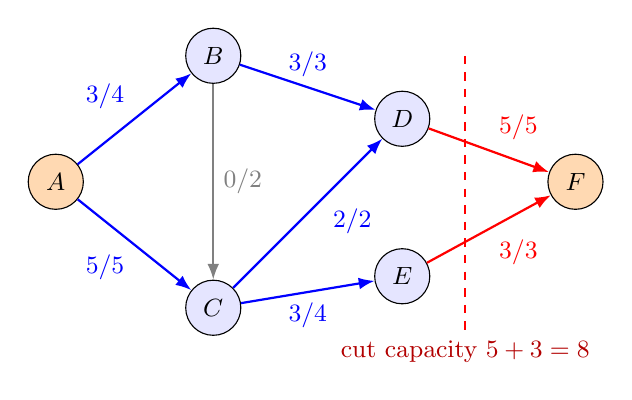
\begin{tikzpicture}[every node/.style={font=\small}, >={Latex[length=2mm]}, v/.style={draw, circle, fill=blue!10, minimum size=7mm, inner sep=0pt}]
	\node[v, fill=orange!30] (A) at (0,0) {$A$};
	\node[v] (B) at (2,1.6) {$B$};
	\node[v] (C) at (2,-1.6) {$C$};
	\node[v] (D) at (4.4,0.8) {$D$};
	\node[v] (E) at (4.4,-1.2) {$E$};
	\node[v, fill=orange!30] (F) at (6.6,0) {$F$};
	\draw[->, thick, blue] (A) -- (B) node[midway, above left] {$3/4$};
	\draw[->, thick, blue] (A) -- (C) node[midway, below left] {$5/5$};
	\draw[->, thick, gray] (B) -- (C) node[midway, right] {$0/2$};
	\draw[->, thick, blue] (B) -- (D) node[midway, above] {$3/3$};
	\draw[->, thick, blue] (C) -- (D) node[pos=0.6, below right] {$2/2$};
	\draw[->, thick, blue] (C) -- (E) node[midway, below] {$3/4$};
	\draw[->, thick, red] (D) -- (F) node[midway, above right] {$5/5$};
	\draw[->, thick, red] (E) -- (F) node[midway, below right] {$3/3$};
	\draw[red, dashed, thick] (5.2,1.6) -- (5.2,-1.9);
	\node[red!70!black, anchor=north] at (5.2,-1.9) {cut capacity $5+3=8$};
	\end{tikzpicture}
\end{document}
